\chapter{多分支因子模型推理框架方案设计}

高频交易场景有因子模型低延时推理的需求,本文针对多分支因子模型的模型结构和业务场景的计算要求,本文提出了多分支因子模型推理框架,从而显著降低多分支因子模型的推理延时。
本章将首先详细阐述多分支因子模型推理框架的总体设计方案,讲述框架的架构设计和基本功能,
随后针对高频交易场景中业务需求的单样本,低延时,多分支等特点,从内存管理和系统配置、算子调优与绑定到分支优化加速的角度更细粒度地介绍优化方法和加速算法设计。
\section{总体设计方案}

因子模型的部署推理过程可以被抽象分为静态预处理和动态运行两个紧密关联且分工明确的阶段。
\begin{figure}[h]
    \centering
    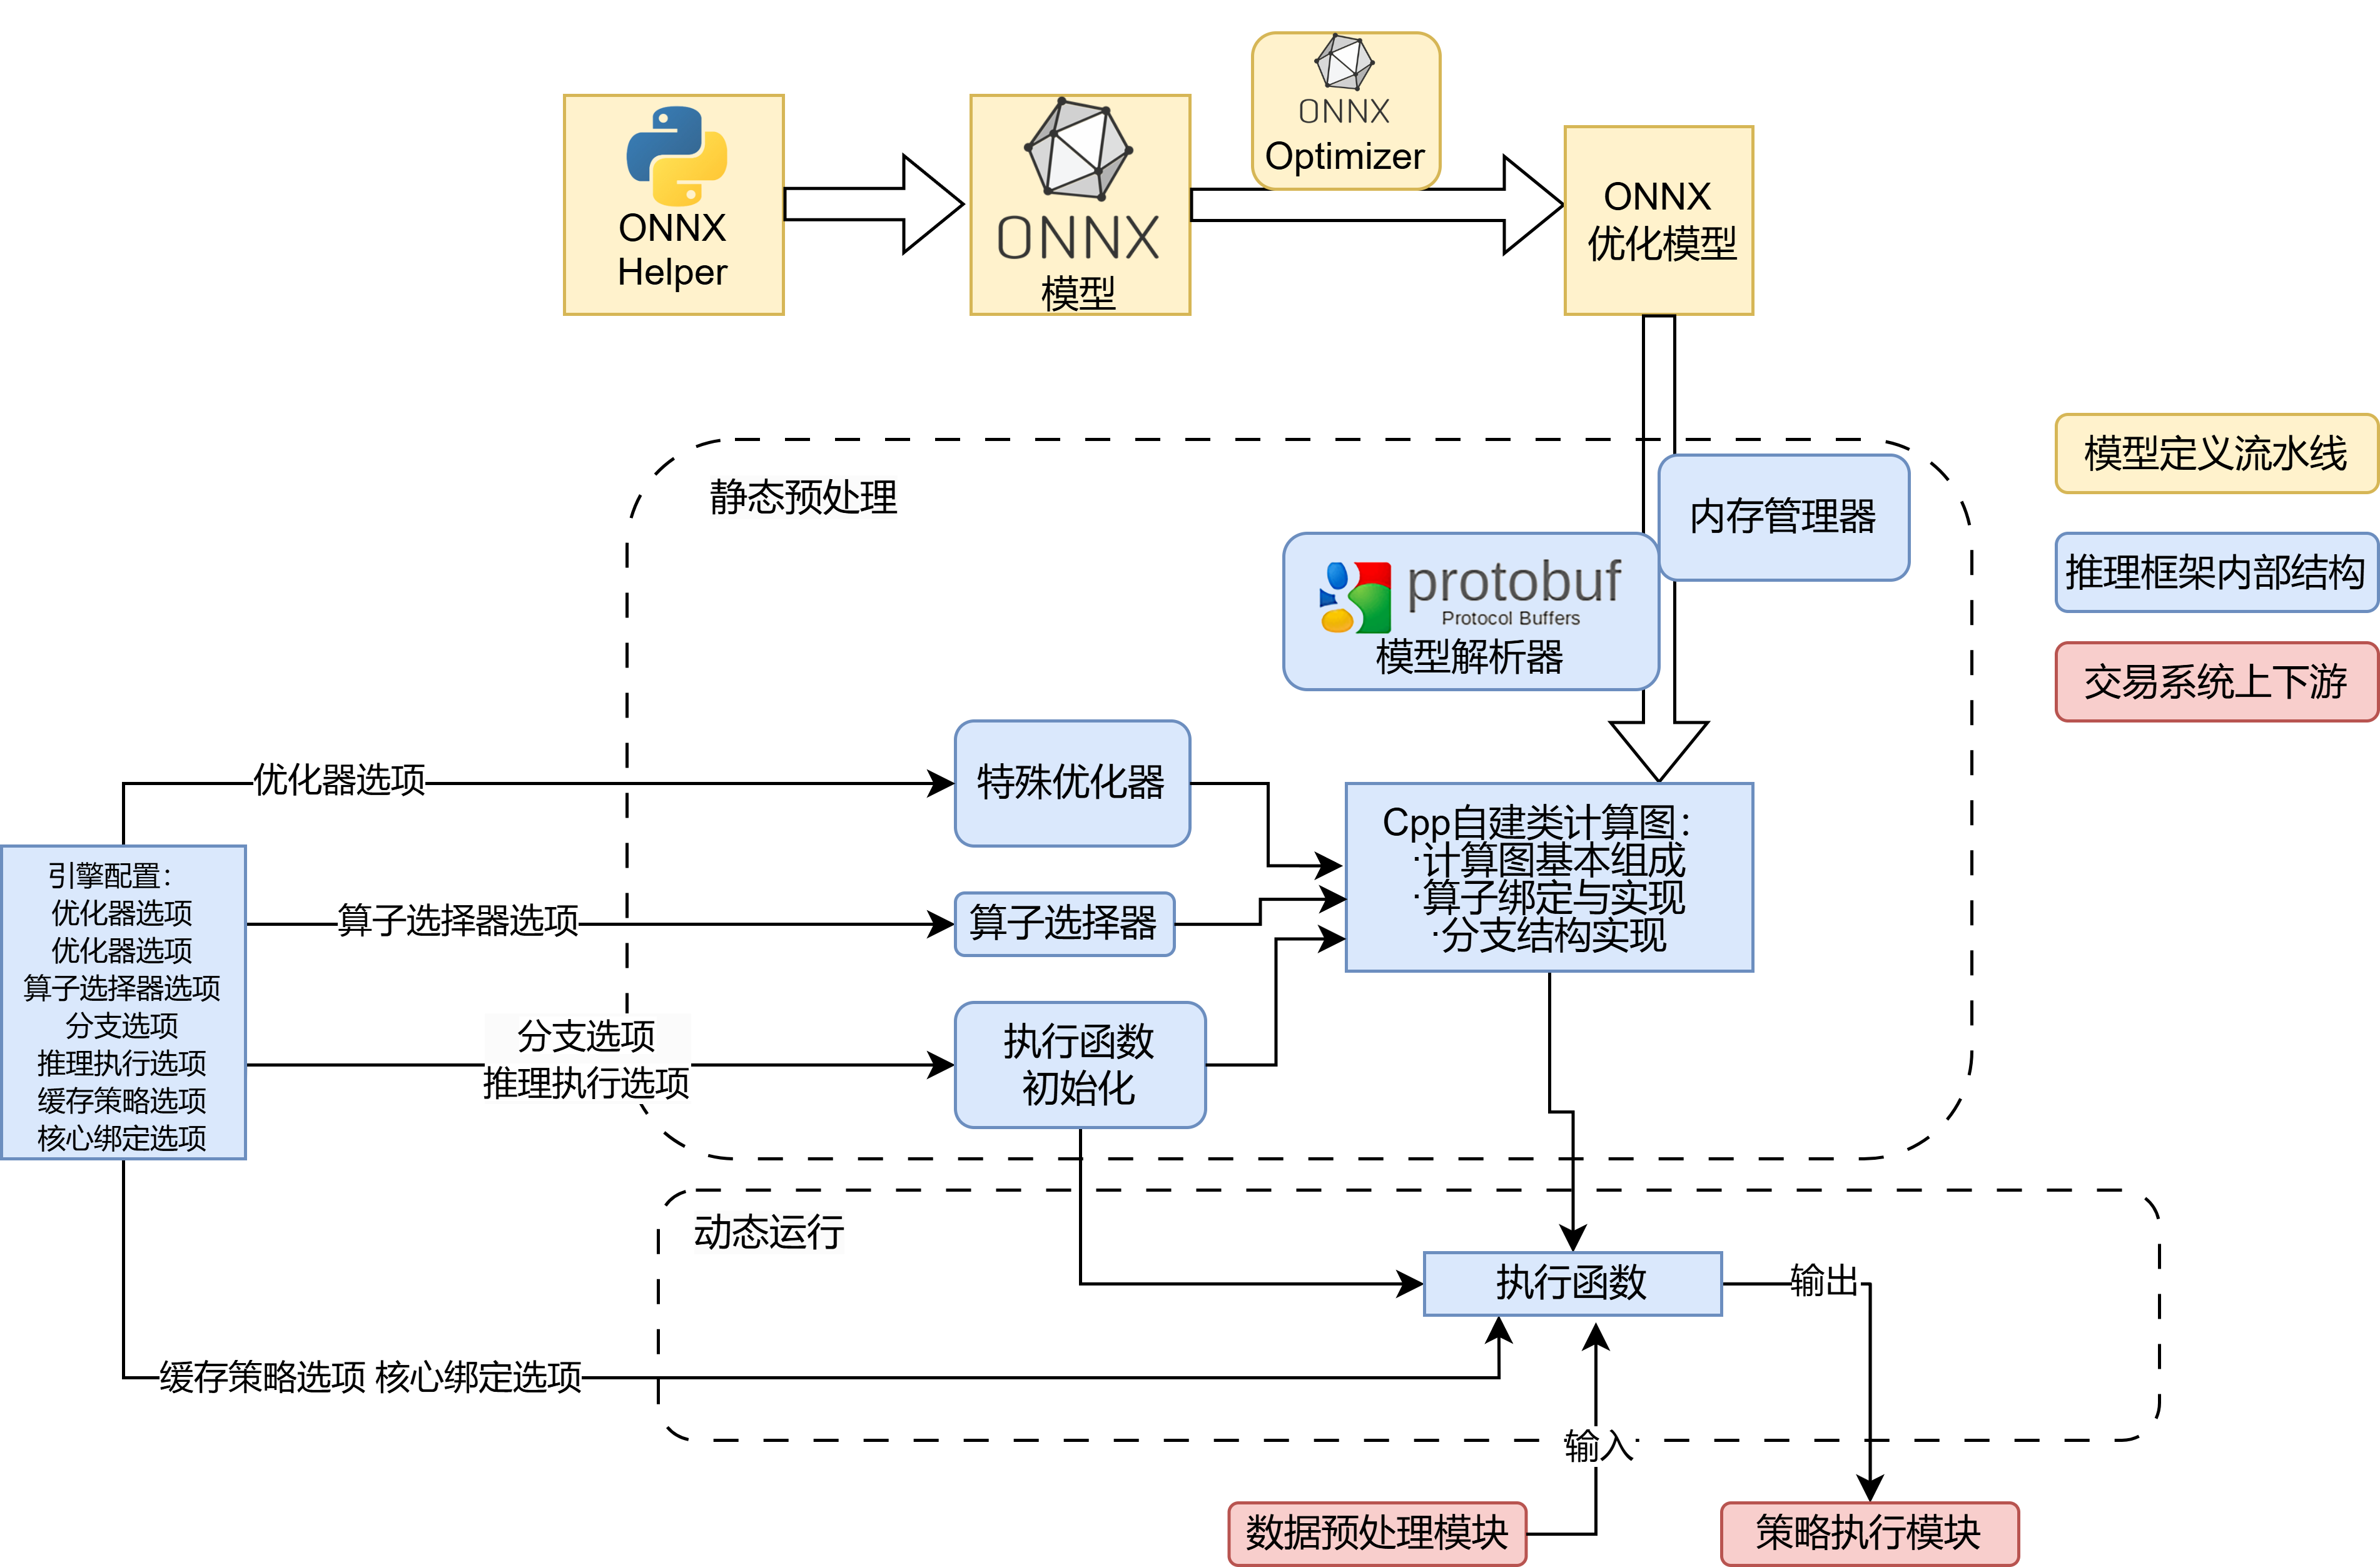
\includegraphics[width=0.9\textwidth]{image/chap03/cnframe.png}
    \caption{框架整体设计}
    \label{fig:cnframe}
\end{figure}
其中静态预处理阶段的核心过程在于结合设备参数、模型计算图等静态信息实施的多方面优化。
此阶段通过采用Protobuf这一高效的序列化工具来解析ONNX格式的机器学习模型,并以此使用自建类对象完成模型计算图重建。
此过程确保了模型拓扑结构和包含信息的完整性,同时为后续优化方案的开发提供对象基础和拓展空间。
随后框架通过自定义的优化模块串行执行优化路径。
通过配置优化路径选项,开发者得以选择性地向优化模块引入各类优化路径,例如:
“无效算子消除”优化路径能够识别并删除对模型最终输出结果无贡献的算子节点,从而有效简化计算图的结构;
“算子融合”优化路径将多个在逻辑上相连、功能上趋近在的算子进行合并,以此减少推理过程中的冗余访存和计算开销;
“模型剪枝”优化路径通过去除模型计算图中的冗余节点与边来削减模型规模,从而降低内存负担同时有效减少模型推理计算量;
“模型量化”优化路径则将模型中的高精度数据类型转换为低精度类型如FP32转换为FP16,在保证模型性能损失可接收的前提下,极大提升计算效率。
通过上述优化模块中优化路径的执行,推理框架能够对计算图独立开展优化,产生独立于其他优化措施的垂直优化效果。
此外,静态预处理阶段还包含算子根据硬件环境进行调优的过程。
这包括获取目标设备的硬件配置细节,包括指令集支持、缓存架构等关键参数,并依据这些信息对计算图涉及的算子进行针对性的调优。
静态预处理过程也包含对于动态运行期间缓存机制的初始化支持,
本文提出的因子模型推理框架在静态预处理过程中,会基于配置请求在模型解析步骤后执行分支拓扑分割算法并完成基于分支的计算图重建。
分支拓扑分割算法依据模型的结构特点,将多分支因子模型计算图划分为多个相对独立且易于处理的子图分支,为动态运行期间的缓存机制提供支撑。

而动态运行阶段则侧重对静态预处理之后所形成的各个组成部分进行高效的加载运行。
在此过程中,CPU核心的隔离和绑定操作能够确保框架推理进程绑定在指定核心运行且系统尽可能减少在该核心运行的无关进程,
实现核心计算资源向框架推理进程倾斜,极大减少由于系统进程调度导致的性能损失。
同时,通过动态配置多分支因子模型的分支缓存策略,分支缓存机制能够简化模型推理过程,减少模型推理所需的计算量,从而降低推理延时。

如上所述,本文提出的多分支因子模型推理框架通过为静态预处理与动态运行两个阶段提供细粒度的优化,实现了局部独立优化与模型整体推理效率的协同提升。
将静态预处理与动态运行两个阶段解耦合的设计方案,在工程设计上降低了项目开发复杂度,从而为后续的优化工作开拓空间。
因此本文能够在此基础上,针对性设计实现优化方案以显著提高因子模型推理性能。

\section{内存管理方案}

\begin{figure}[h]
    \centering
    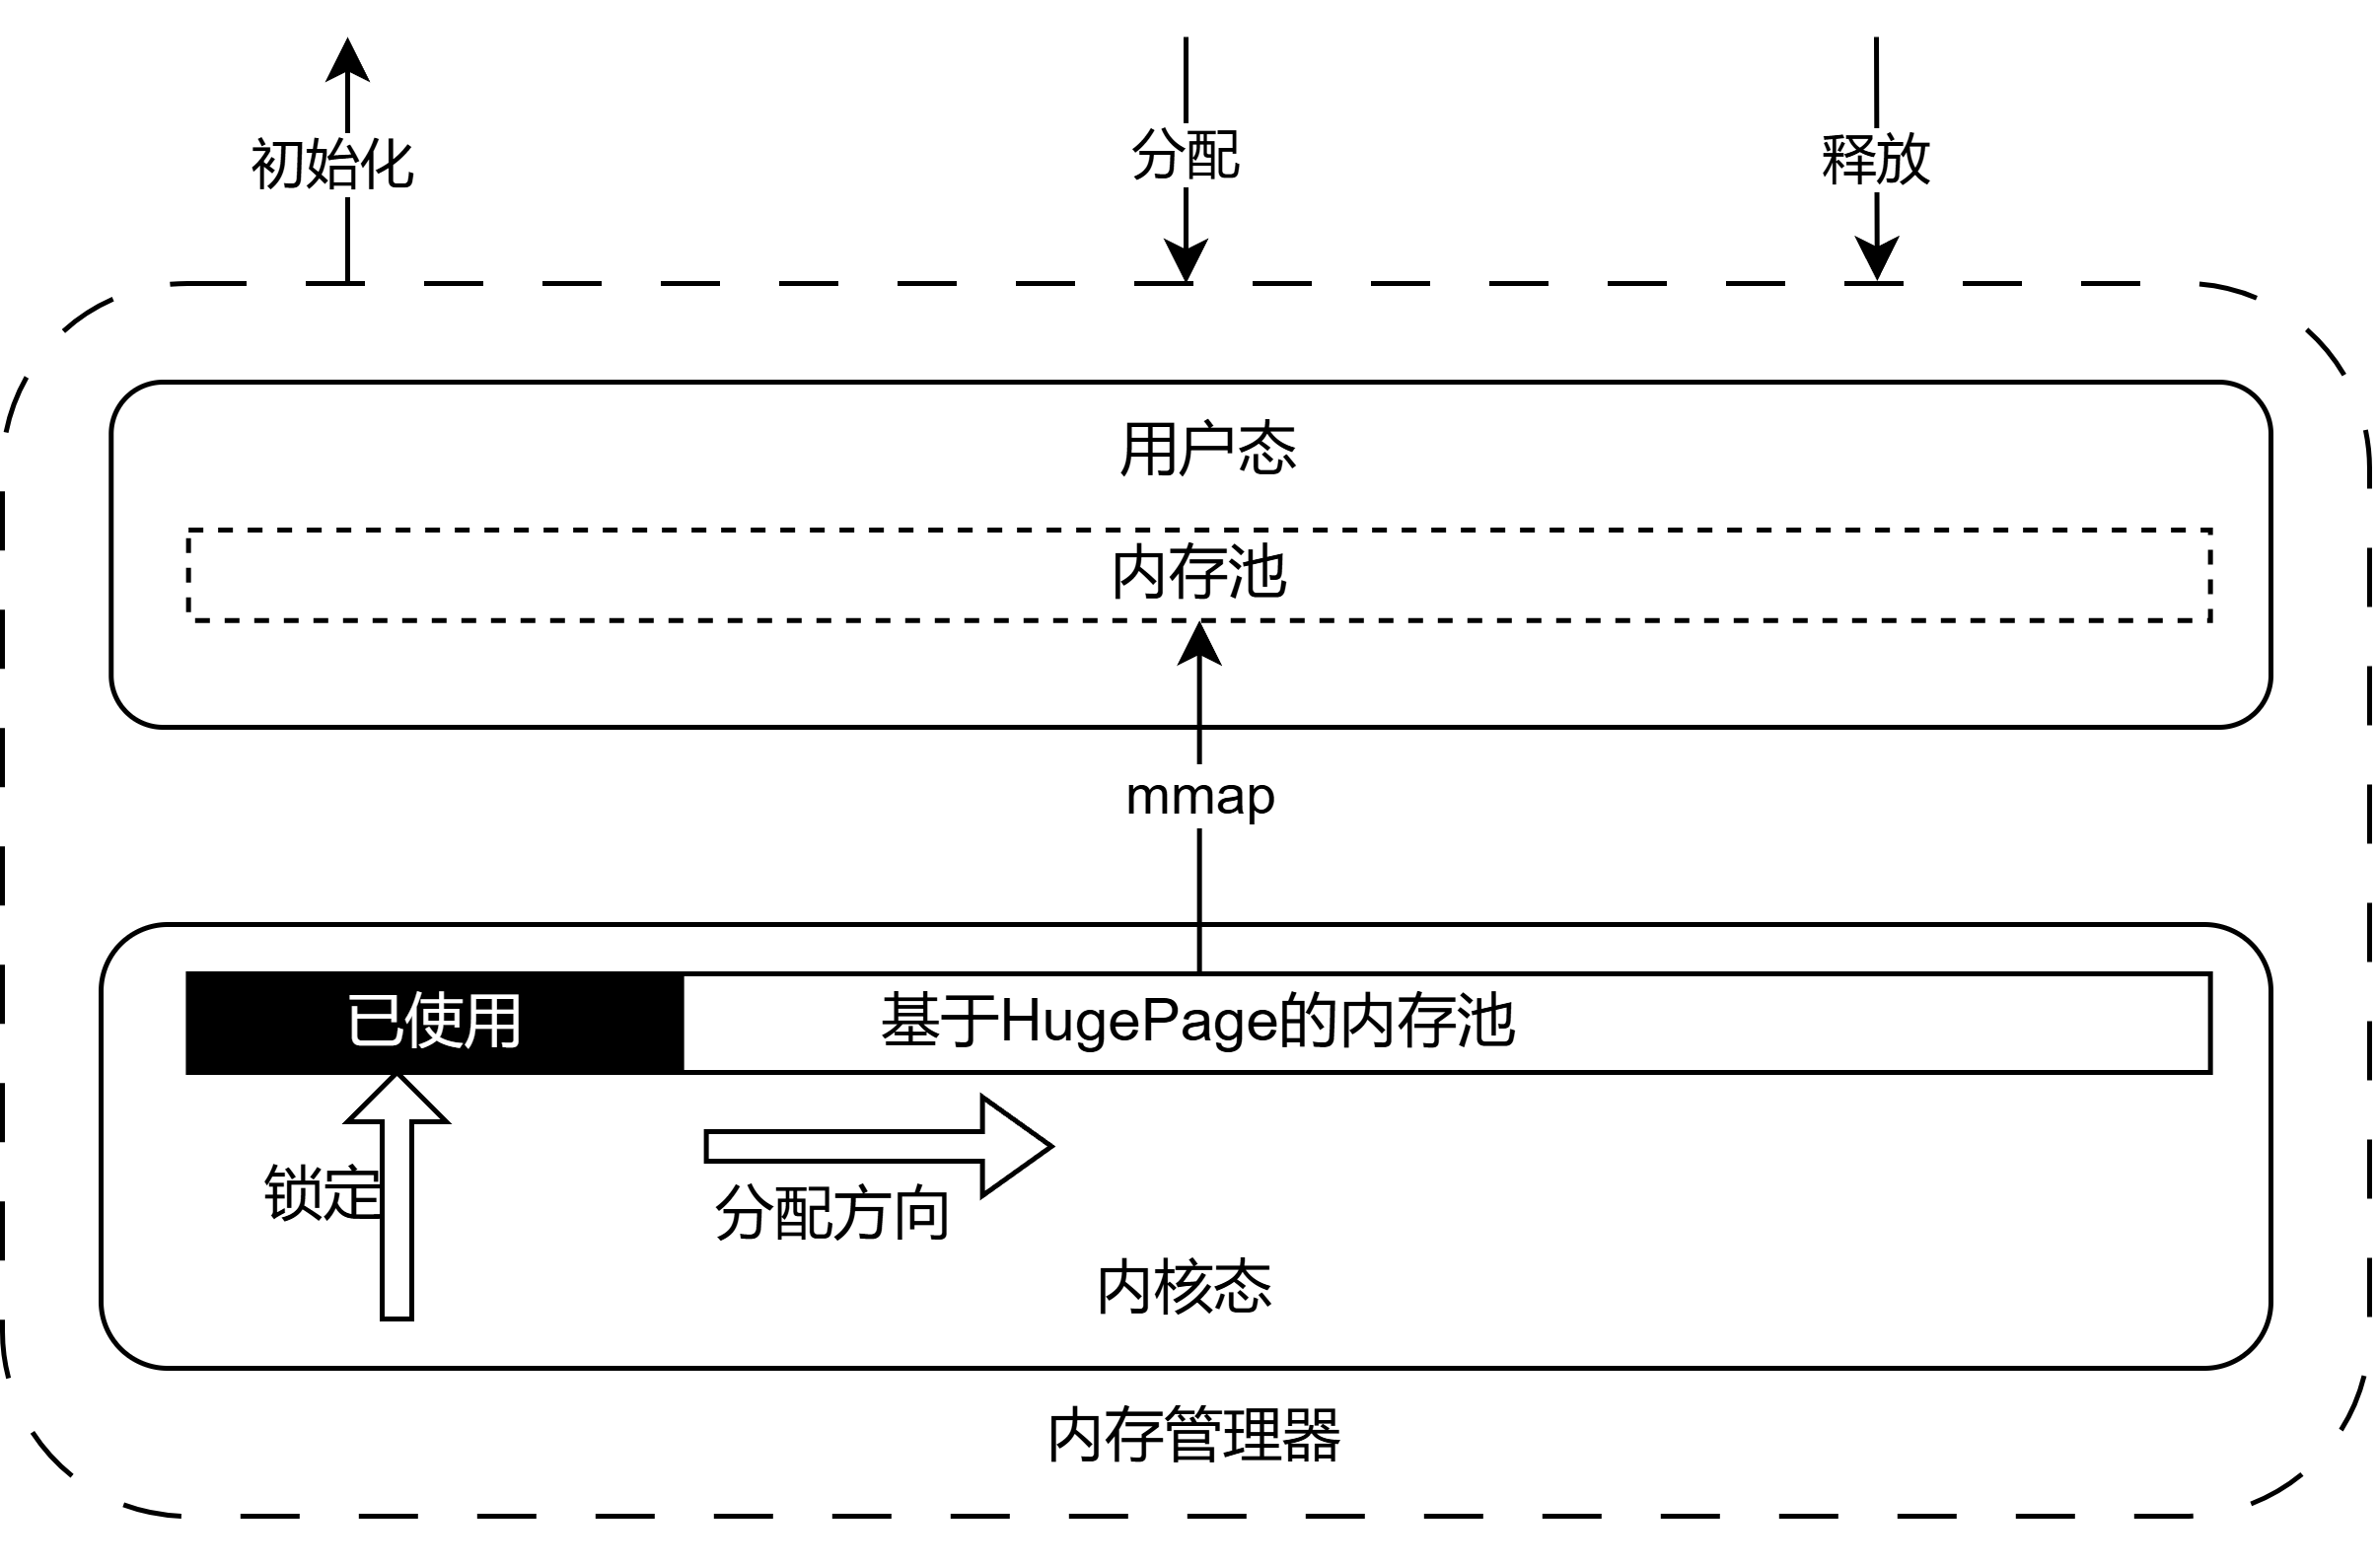
\includegraphics[width=0.9\textwidth]{image/chap03/memma.png}
    \caption{内存管理器示意图}
    \label{fig:memmory}
\end{figure}

低延时交易系统的因子模型推理模块对于访存效率具有很高的要求,多分支因子模型推理框架的优化上限受限于高效的内存管理策略所能带来的访存性能提升。
为了满足高频交易场景下的低延迟推理需求,框架通过内存池和分配器机制相结合,设计实现了一套高效的内存管理方案。

内存池是推理框架内存管理器的核心模块,其主要功能是通过预分配预设大小的内存空间块,并通过分配器设计控制已分配内存的使用权,旨在消除在动态运行阶段由于分配新的内存空间块而导致的延时。
为了最大限度地提高内存访问速度并减少内存碎片,内存池使用 mmap 系统调用来分配基于 Huge Page 的 1GB 内存区域。
Huge Page 作为操作系统本身提供的一种大页内存管理机制,其通过减少页面表条目数量和提高内存访问的TLB命中率来显著提高内存访问速度。
结合mmap操作,从内核态中的大页内存空间得以映射到用户态空间,从而能够被用户态的模型推理框架自由使用。
而就框架本身的两个阶段而言,模型推理所需要的计算图存储空间和张量存储空间,均在静态预处理阶段完成分配,推理过程在动态运行阶段并无其他向量或结构需要重新分配内存空间。
因此相比较现有的内存池,框架中所设计的线性分配内存池并不需要维护一个记录已分配内存的链表结构,只需要各个变量持有其内存起点和内存大小即可。
实际部署中,在静态预处理阶段,框架使用mmap调用分配了一个1GB的大页内存块,并将其映射到用户态的进程地址空间。
内存池通过维护一个指向当前可分配内存起点的指针,使其在每次分配内存时,只需要通过更新该指针的位置来分配连续的内存块,从而有效减少了传统内存分配算法中复杂的链表数据结构和内存碎片复用问题。
内存池的设计还有助于提高系统的可扩展性,便于根据不同的硬件配置和应用场景进行灵活调整,确保在不同环境下实现最佳的内存管理效果。

内存分配器则是内存池对外使用的操作接口,其通过简单维护内存池可分配内存的起点指针将内存池中的内存分配给指定变量。
在静态预处理阶段的模型解析阶段,框架首先通过Protobuf解析Onnx模型,此时通过内存分配器,可以为模型计算图的拓扑结构与计算节点的输入输出张量分配内存。
分配器会结合变量请求的内存大小和可用内存大小,从内存池中分配可用的内存块,其过程如下:
分配器检查内存池中是否有足够的连续内存块可供分配;
如果有,分配器就会更新指向内存池可分配内存起点的指针,并将内存块分配给张量。
如果没有,分配器报错提示内存池无可用内存。

框架会在静态预处理阶段结束时固定已被内存分配器分配的内存空间。
这一策略得益于高频交易场景下模型输入输出张量和计算图拓扑结构均具有相对固定大小,
这意味着推理框架在静态预处理阶段完成后,内存池中的已分配内存将固定在内存中不可回收,从而了保证动态运行阶段对已分配内存的高效访存操作。
推理框架也将分配的内存锁定到物理内存,防止操作系统将这些内存页交换到磁盘。
这种方案有效降低了内存访问的延迟,同时提高了系统稳定性,使框架在高负载下,也能有效消除因内存交换而造成的缺页中断延时。
从系统设计的角度看,固定内存分配策略提高了系统的可预测性,为监控和优化内存使用情况提供了良好的工具,保证了系统的长期稳定运行。

通过内存池和分配器设计,结合Linux系统的内存映射,大页内存和内存锁定机制,框架的内存管理系统得以为多分支因子模型的推理过程提供透明的高效内存访问,为多分支因子模型推理框架的优化奠定了良好的基础。

\section{算子调优与绑定}
在高频交易业务场景下,程序自动交易链路的全过程对延时的要求极为苛刻,关键路径的最大延时必须被约束在数十乃至数微秒。
低延时要求的满足与否决定了量化策略是否能够在预期价格位置执行交易。
因此,作为关键路径中延时的主要来源,因子模型的计算过程必须充分利用硬件性能以减小延时,
对于实际的CPU部署场景,调优算子以提高硬件利用率是模型推理优化开发中必不可少的环节。

在此前提下,框架提供了算子调优与绑定的简易步骤,加速了框架应用于目标硬件的部署实践。
首先,框架在Blaze HPC编译过程中结合Intel MKL、AMD AOCL等数学库与CPU架构信息,如各级缓存大小、指令集等,从而在算子性能本身提供最优实践。
针对不同CPU的指令集特性支持,结合可用的指令集特性与实际的设备部署环境进行综合方案设计是算子性能调优的重点。
SIMD作为CPU向量化数据处理的关键技术,而近年来以AVX2和AVX-512指令集为提高SIMD运算的关键,其能够显著提升CPU对于数据的并行处理能力。
其中AVX2支持256位的向量化操作,AVX-512则进一步扩展到512位,后者在理论上能够有效提高计算效率。
然而在实际应用中,AVX-512指令集应用带来的性能提升可能是受限的,尤其是在特定型号的CPU上。
AMD EPYC CPU,其虽然通过CCX/CCD的核簇封装有效提高了局部的核心密度,但是同样也带来了严重的散热障碍。
虽然其支持AVX-512指令集,但在多数计算密集场景下,使用AVX-512指令集的二进制应用大概率会导致CPU积热,从而触发CPU全核心降频。
低延时交易系统整体的延时因此升高,反而降低了整体性能,得不偿失。
为了避免这种情况,优化策略中需要根据具体的CPU型号和应用场景灵活选择指令集。
例如对于Intel 四代Xeon与FP16的数据操作,应当选择AMX指令集用于快速矩阵操作;而对于AMD EPYC处理器的FP32数据操作,应当充分考量其实际部署的机身物理环境,选择性使用AVX2或AVX-512指令集编译应用。

其次,对于Blaze HPC不支持的进一步优化,在部署框架过程中,框架通过Selector类可以综合计算需求和CPU信息来动态绑定算子。
例如,Intel GEMM JIT对于小规模浮点数矩阵乘有显著加速效果,框架通过判定指定节点的计算类型和规模,可将该节点算子绑定到Intel GEMM JIT。
因此,算子绑定过程具有极大的可拓展性,对于先进的计算优化也可以通过简单的拓展开发进行快速适配。
同样,模型经过静态优化模块可以产生节点的融合,对于此类非常规的算子,BLAS通常不能提供支持,但框架仍然支持通过简易的拓展开发实现手写算子,只需要使用CPU定制编译器如ICPX等进行目标架构的针对性优化即可。
通过上述算子的调优与绑定过程,算子执行得以充分利用硬件的性能,极大提高了因子模型的推理效率。

\section{分支拓扑分割算法}

\begin{figure}[h]
    \centering
    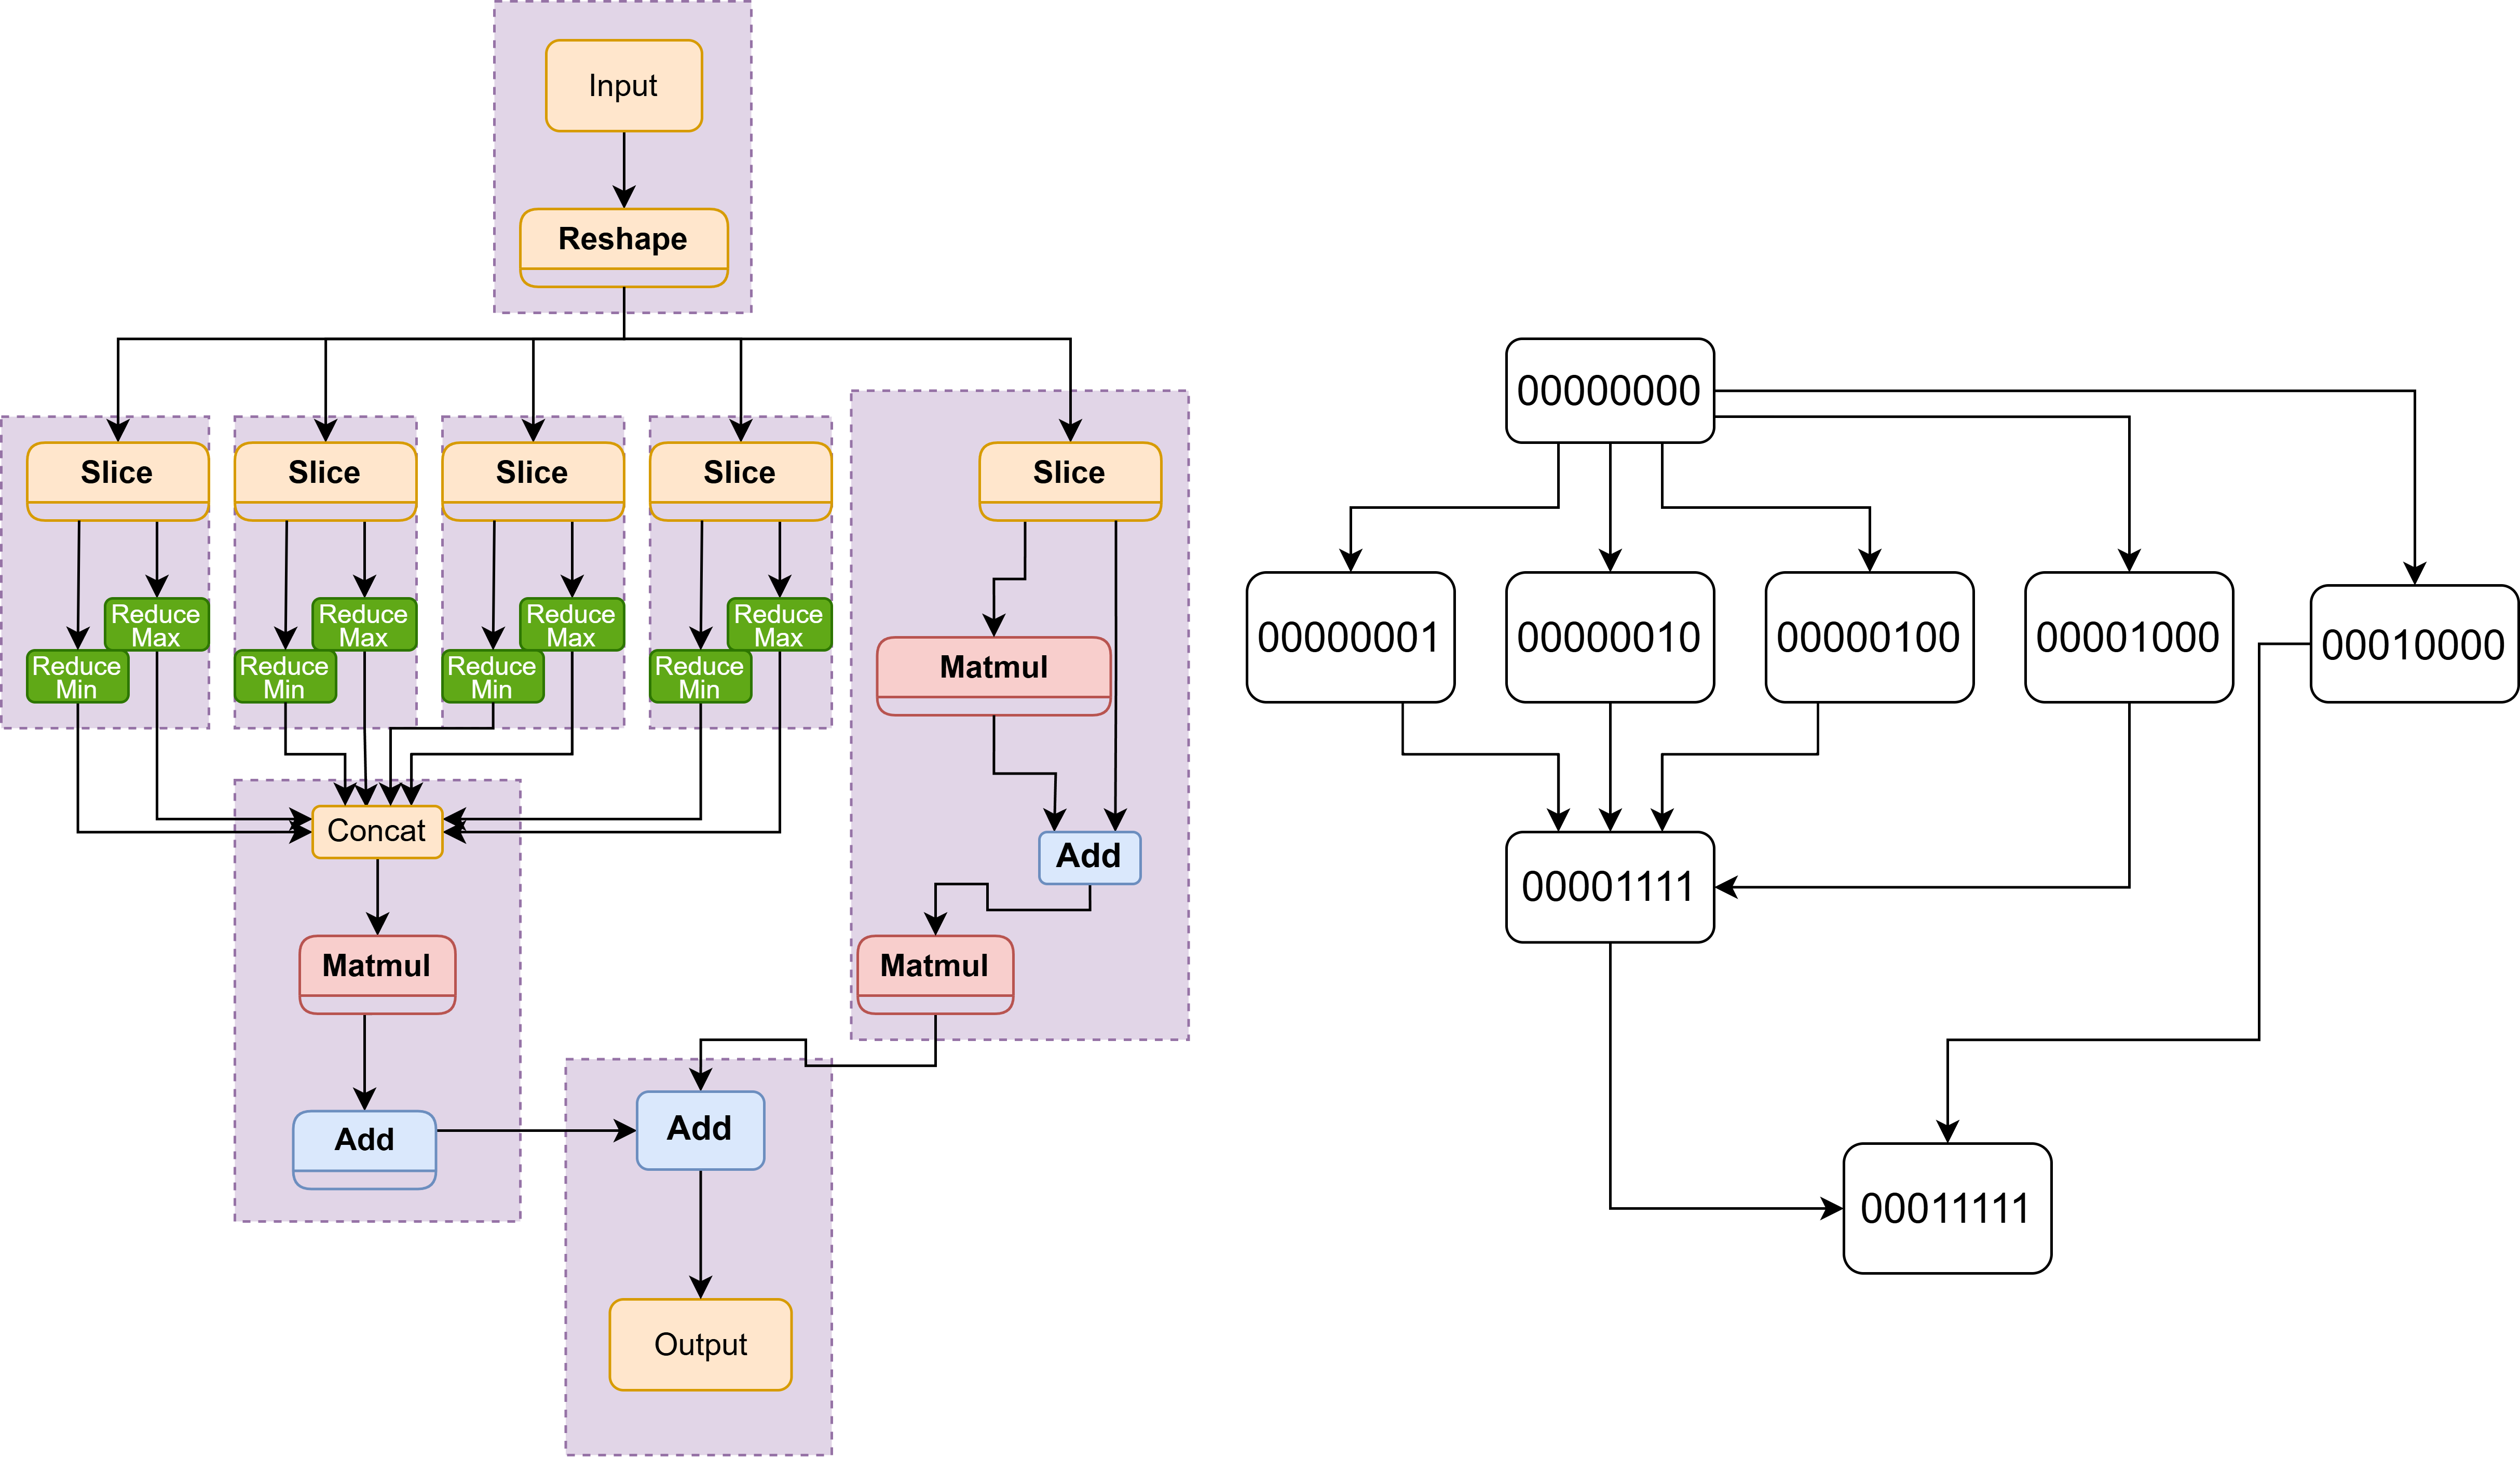
\includegraphics[width=0.9\textwidth]{image/chap03/modelg.png}
    \caption{分支拓扑分割算法中以分支为单位的计算图重建与分支位标记示意图}
    \label{fig:branchs}
\end{figure}
在数据预处理模块更新行情数据库从而计算更新行情统计数据之后,这些统计数据通过拼接操作合并为一维向量输入到多分支因子模型中执行推理计算,其在进入模型后通过切片操作被切分到不同分支中独立处理。
尽管针对不同交易品类而设计的多分支因子模型在具体的算子设计上存在较大差异,
但从模型整体的拓扑结构而言,各个分支在经过初步处理后,都会通过通用矩阵乘法以将低维度的输入统计特征映射到高维空间中,在此操作后各分支之间通过计算操作如向量加或矩阵乘实现不同分支间的逐级合并,最终得到一个输出用以指示行情特征。
多分支因子模型的结构就类似于从叶子到根的树状收敛结构,这一独特的拓扑结构使其表现出与其他模型不同的优化潜力。

为了充分利用多分支因子模型的输入模式与结构特征,框架设计了分支拓扑分割算法以实现在多分支因子模型中分割得到分支结构并以分支为基本单位重建计算图。
而以分支为基础的重建有助于充分展示模型的拓扑结构,这也为在动态运行过程中启用的分支缓存机制提供了基础对象的初始化支持。
在工程设计方面,分支拓扑分割算法得到的分支结构为多分支因子模型优化提供了除图和节点以外的另一个拓扑描述粒度。
在优化方案的设计过程中,分支结构为计算图在新的抽象层拓展获得了更多的优化空间。
算法流程如算法\ref{algo:branch_topology_partitioning}所示。
\begin{algorithm}[h]
    \KwIn{计算图G,输入节点集合InputNodes,分支初始节点集合BranchStartNodes}
    \KwOut{以分支为单位的计算图结构PartitionedGraph}
    \textbf{初始化:}\;
    \For{输入节点$InputNode$ in $InputNodes$}{
        \For{切片操作$SliceOpNode$ in $InputNode$.$ChildNodes$}{
            为每个分支初始节点分配一个唯一的位标记$BitMask$,如$BitMask = 1 << index$\;
        }
    }
    
    \textbf{深度优先搜索标记传播:}\;
    \For{分支初始节点$BranchNode$ in $BranchStartNodes$}{
        初始化当前分支标记$CurrentBitMask = BranchNode$.位标记\;
        \textbf{深度优先搜索:}\;
        \For{子节点$ChildNode$ in $BranchNode$.$ChildNodes$集合}{
            $ChildNode$.$BitMask |= CurrentBitMask$\;
            递归地对$ChildNode$的子节点进行相同操作\;
        }
    }
    \textbf{深度优先搜索计算图重建:}\;
    初始化当前位标记$CurrentBitMask = 0$\;
    当前节点为$CurrentNode = InputNodes$\;
    当前分支为$InputNodes$组成的初始分支$CurrentBranch = InputBranch$,然后深度优先搜索子节点;
    \For{$Node$ in $CurrentNode$.$ChildNodes$}{
    \If{$Node$.$BitMask$ != $CurrentNode$.$BitMask$}{
        创建新的分支$NewBranch$;
        $CurrentBranch$.$ChildBranch$加入$NewBranch$;
        $CurrentBranch$ = $NewBranch$;
        $CurrentNode$.$BitMask$ = $Node$.$BitMask$
    }
    将$Node$添加到$NewBranch$;
    递归地对$Node$.$ChildNodes$进行相同操作;
    }
    将所有分支整合到PartitionedGraph中;

    \caption{分支拓扑分割算法}
    \label{algo:branch_topology_partitioning}
\end{algorithm}

这样,在模型推理过程中,可以针对每个分支进行独立的优化操作,例如缓存管理、资源分配等,从而拓展优化空间。
利用位运算标记分支,可以将以节点为单位的计算图重建为以分支为单位的计算图,用以支持之后的分支缓存算法加速计算。

\section{分支缓存机制}

\subsection{基于实时行情的分支缓存}

在实际的高频交易场景中,在最高级别的实时行情(Full Tick)下,该交易品类下所有交易操作都会实时发送到低延时系统更新和处理。
此类行情更新虽然具有优越的实时性和最详尽的行情数据,但是另一方面任意交易者的所有操作都会触发交易系统的一轮执行,带来了极高的计算压力。
然而,并不是所有交易操作都会对因子模型的特征输入产生影响,例如偏离最优成交价格的预埋单,并不会影响因子模型对于行情的基本特征提取。
这意味着尽管交易因子模型仍然必须在行情更新时进行推理,但是其部分特征输入在多数情况下不受行情数据中噪声操作更新影响。
而此类对行情变化不敏感的特征输入对应部分分支的计算过程就存在优化空间。

框架使用分支拓扑分割方法基于分支重建了模型计算图。
通过在分支推理函数中添加分支输入与缓存的上一次输入匹配函数,可以在缓存命中的条件下可以将上次计算结果返回输出。
此类方法不仅对于输入特征本身的数据格式没有特殊要求,
而且在高频场景下每秒的数万次行情操作更新中,多数操作实际为行情噪声,仅有少数趋势成交导致行情特征数值变化从而影响因子模型推理。
\begin{figure}[h]
    \centering
    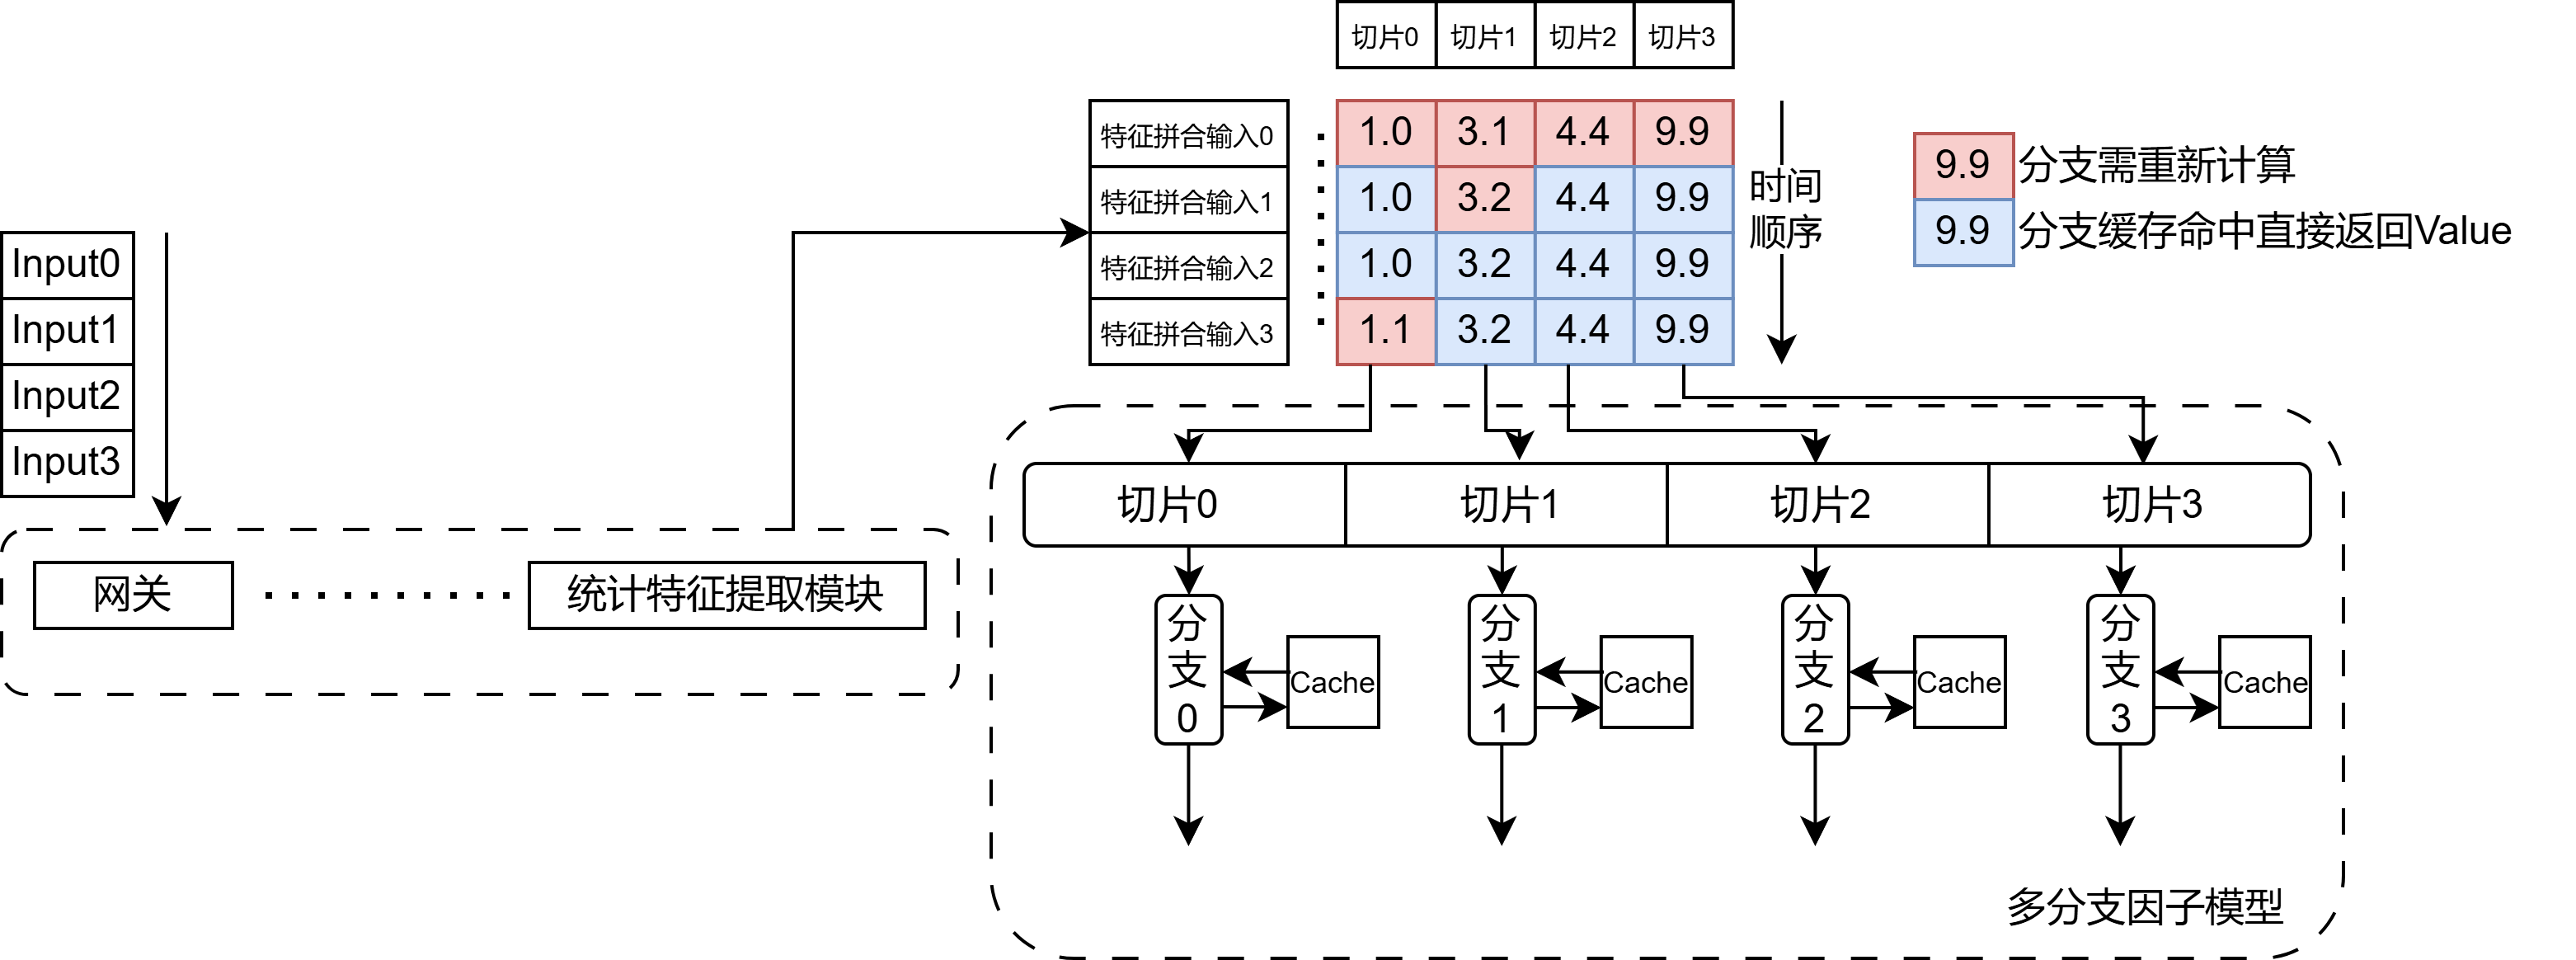
\includegraphics[width=1\textwidth]{image/chap03/high.png}
    \caption{实时行情中缓存加速}
    \label{fig:hole1}
\end{figure}

\subsection{基于可枚举输入特征的预计算分支缓存}

多分支因子模型的拼接输入,其由多个行情统计特征组成,而统计特征在某些情况下由单一数据构成,
因此相较于其他机器学习模型的复杂输入,多分支因子模型的分支输入具有可枚举性。
以交易指标中的当前成交价格为例,在期货交易市场上,交易所会为每个交易品种设定一个最小的价格波动单位,这直接约束了交易价格的取值范围为有限离散值。
而对于多数交易日,除非出现偶发的黑天鹅事件,否则单个交易日内的价格波动会在一定局部范围内。
这里以沪铝 2503 合约为例,其最小价格波动单位为 5 元/吨,在实际交易中,单个交易日内其价格波动极少超过 500 元。
结合这一特点,框架在交易日开盘前基于盘前价格预先计算并缓存了包含涨跌情况的 100 个成交价格输入值和对应的分支推理输出。
这样,在整个交易日中,模型可以直接从缓存中提取预先计算的结果,从而有效节约计算时间,降低推理延时。
同时,框架为该分支所分配的缓存大小也在接受范围内,并没有占用过多内存。
同样,对于低精度格式(如 FP16)的因子输入,由于大多数市场特征都是单值的,因此可以预先计算分支输出,并通过枚举 FP16 的所有可能值来构建缓存。

为了实现这一优化,多分支因子推理框架在执行上述分支拓扑分割算法后,在动态运行阶段为每个分支配置和引入缓存机制。
使得当输入的市场数据与缓存中的数据相匹配时,模型能够直接从缓存中检索预计算的输出,并将其传递给后续分支结构。
缓存机制通过将分支推理简化为哈希表查询过程,有效避免了冗余计算,降低了模型整体的推理延时。
\begin{figure}[h]
    \centering
    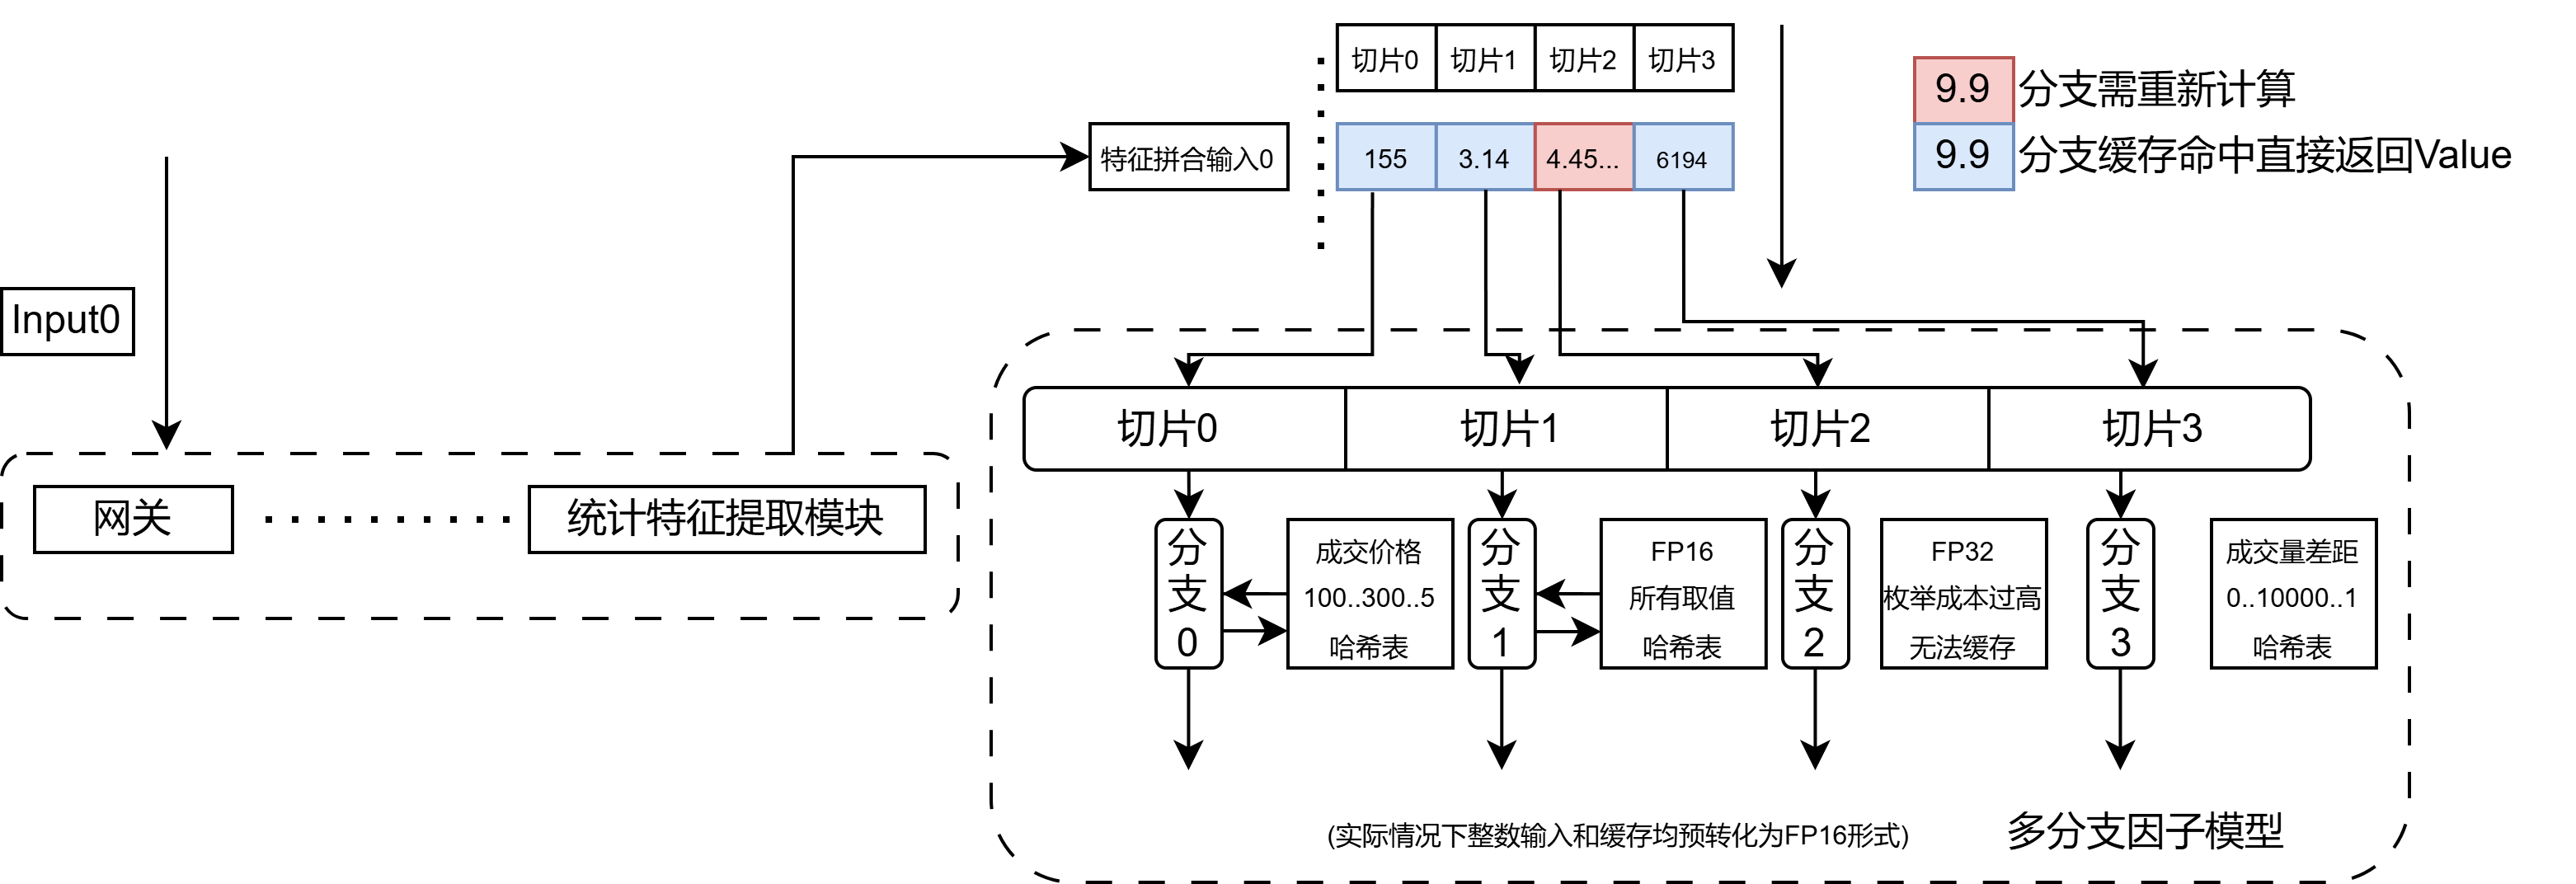
\includegraphics[width=1\textwidth]{image/chap03/precom.png}
    \caption{通过预计算缓存加速}
    \label{fig:hole2}
\end{figure}

\subsection{缓存机制的选取}

实现缓存机制尽管在多数情况下能够实现分支计算过程的简化加速,
但是对于高频交易系统,缓存机制作为分支抽象层的附加实现,需要考虑在缓存未命中条件下的执行延时增加。
而在CPU缓存和系统内存缓存中常用的LRU与FIFO等机制,其需要维护动态缓存池,
相比较匹配上一次输入和预计算固定缓存查询具有较高的延时成本,即便通过维护动态缓存池可能有效提高缓存命中率,但是无缓存命中情况下的推理延时显著增加。
因此缓存机制只使用匹配上一次输入和预计算固定缓存查询两种高效缓存方法,其相比较原推理过程不仅通过缓存命中大幅减少推理延时,在无缓存命中情况下的推理延时几乎没有增加。

因此只有选择适合业务场景的缓存替换机制才能够有效降低推理延时,这要求综合考虑市场数据的特点与模型的输入模式。
通过分析模型部署实例中采集的市场数据流并结合模型的输入模式进行不同缓存策略的组合测试,才能够达到缓存机制下模型推理的最低延时。
在实际的缓存策略选取中,可以基于分支结构针对不同的分支,选择性地组合各种缓存策略,从而能够使模型整体推理达到最佳性能。
而不同的市场交易品类,市场数据的特征会发生显著的变化,例如农产品具有显著的周期性,而股票则具有更加复杂的驱动因素。
因此需要针对交易品类对缓存策略进行评估调整,以确保其能够始终适应当前品类波动的市场环境。
缓存机制同时需要满足交易系统的实时性和稳定性要求,因此缓存机制的设计实现还需要充分考虑分支输入数据和输出数据的准确一致性,需要考虑不同哈希实现的不同操作效率,避免由于缓存策略失效导致实例挂起。
伴随交易规模的扩大和市场数据量的累加,缓存机制的开发同样要求高可拓展和可维护性,以确保交易系统保持高效性能的同时长期稳定运行。
